\begin{figure}[h]
\centering 
\includegraphics[scale=0.3]{images/Angular.png}
\caption{Angular.js logo}
\end{figure}
\noindent AngularJS is a structural framework for dynamic web apps. It lets you use HTML as your template language and lets you extend HTML's syntax to express your application's components clearly and succinctly. Angular's data binding and dependency injection eliminate much of the code you would otherwise have to write. And it all happens within the browser, making it an ideal partner with any server technology.

Angular is not a single piece in the overall puzzle of building the client-side of a web application. It handles all of the DOM and AJAX glue code you once wrote by hand and puts it in a well-defined structure. This makes Angular opinionated about how a CRUD (Create, Read, Update, Delete) application should be built. But while it is opinionated, it also tries to make sure that its opinion is just a starting point you can easily change.

\begin{figure}[h]
\centering 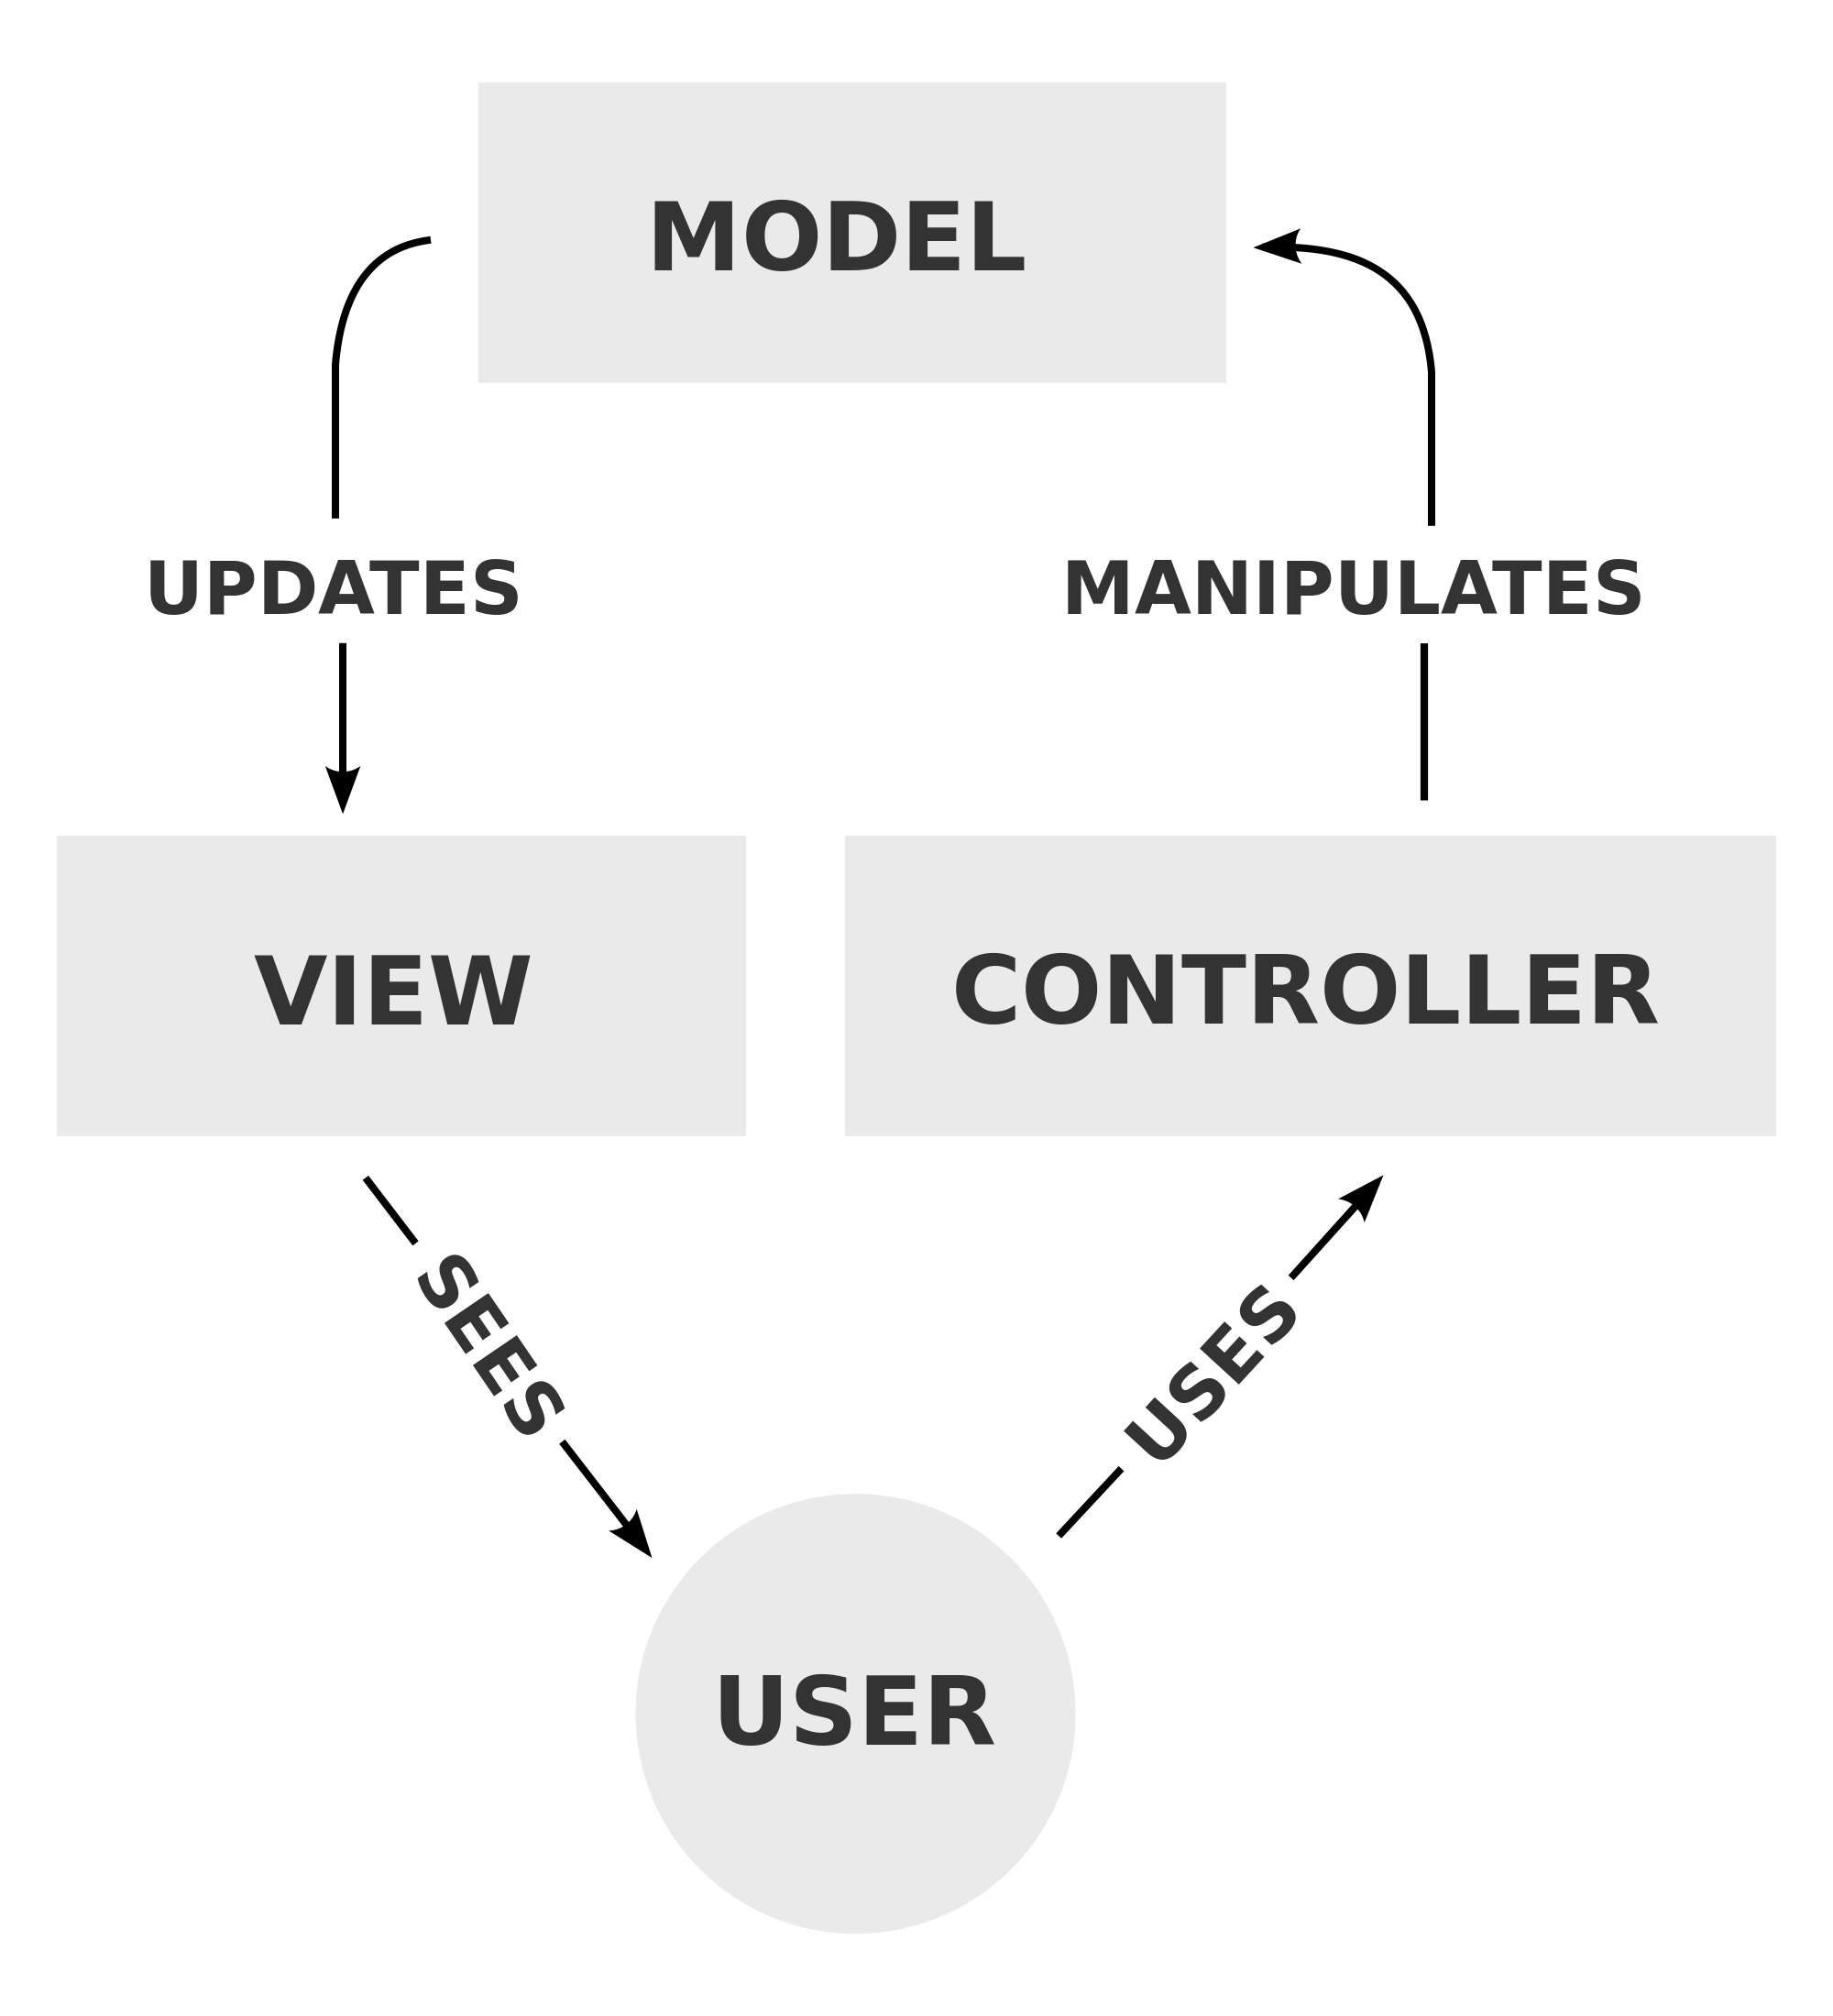
\includegraphics[scale=0.1]{images/mvc.png}
\caption{Model View Controller}
\end{figure}

\subsection{Features of Angular}
\begin{itemize}
\item It is a very good idea to decouple DOM manipulation from app logic. This dramatically improves the testability of the code.
\item It is a really, really good idea to regard app testing as equal in importance to app writing. Testing difficulty is dramatically affected by the way the code is structured.
\item It is an excellent idea to decouple the client side of an app from the server side. This allows development work to progress in parallel, and allows for reuse of both sides.
\item It is very helpful indeed if the framework guides developers through the entire journey of building an app: From designing the UI, through writing the business logic, to testing.
\item It is always good to make common tasks trivial and difficult tasks possible.
\end{itemize}
